\documentclass[12pt]{article}
\usepackage{header}
\usepackage[a4paper, bottom=3.5cm, top=2.5cm, left=3cm, right=3cm]{geometry}
\sisetup{detect-family = true}

\title{\textsf{\textbf{Entrega 2}: Cadenes de desintegració radioactiva}}
\author{\textsf{Arnau Mas}}
\date{\textsf{23 de Març de 2018}}

\begin{document}
\selectlanguage{catalan}
\maketitle
Considerem la següent cadena de desintegracions
\begin{equation*}
	X \to Y \to Z
\end{equation*}
on Z és un nucli estable i \( X \) i \( Y \) tenen constants de desintegració \( \lambda_X \) i \( \lambda_Y \) respectivament. Suposem que tenim un nombre inicial \( N \) de nuclis.

Tenim que el nombre de nuclis \( X \), \( N_X \), decau com \( -A_X \), on \( A_X \) és l'activitat de \( X \) és a dir, el nombre de desintegracions de \( X \) en \( Y \). Per tant \( \dot{N}_X = -A_X \). El nombre de nuclis de \( Y \)   també decau com \( -A_Y \) on ara \( A_Y \) és l'activitat de \( Y \), és a dir, el nombre de desintegracions de \( X \) en \( Z \). Però, com que \( A_X \) era el nombre de nuclis de \( X \) que es desintegraven en \( Y \), \( N_Y \) també incrementa com \( A_Y \). Per tant \( \dot{N}_Y = A_X - A_Y \). Així doncs, tenint en compte que \( A_X = \lambda_X N_X \) i que \( A_Y = \lambda_Y N_Y \) tenim el següent sistema d'equacions diferencials:
\begin{equation} \label{eq:eqs diferencials}
	\left.
		\begin{aligned}
			\dot{N}_X &= -\lambda_X N_X \\
			\dot{N}_Y & = \lambda_X N_X - \lambda_Y N_Y
		\end{aligned}	
	\right\}.
\end{equation}
En forma matricial podem escriure
\begin{equation} \label{eq:eqs diferencials matriu}
	\begin{pmatrix}
		\dot{N}_X \\
		\dot{N}_Y 
	\end{pmatrix}
	=
	\begin{pmatrix}
		- \lambda_X & 0 \\
		\lambda_X & -\lambda_Y 
	\end{pmatrix}
	\begin{pmatrix}
		N_X \\
		N_Y
	\end{pmatrix}.
\end{equation}
La matriu d'aquest sistema té valors propis \( -\lambda_X \) i \( -\lambda_Y \), per tant diagonalitza. Per valor propi \( -\lambda_X \) el sistema es redueix a \( \dot{N}_X = -\lambda_X N_X \) i \( N_Y = \frac{\lambda_X}{\lambda_Y - \lambda_X} N_X \). I pel valor propi \( -\lambda_Y \) tenim \( \dot{N}_Y = -\lambda_Y N_Y \) i \( N_X = 0 \). Així doncs, la solució general del sistema és 
\begin{equation} \label{eq:sol general}
\left.
	\begin{aligned}
		N_X(t) & = Ae^{-\lambda_X t} \\
		N_Y(t) & = A\frac{\lambda_X}{\lambda_Y - \lambda_X}e^{-\lambda_X t} + Be^{-\lambda_Y t}
	\end{aligned}
\right\}.
\end{equation}

Si a \ref{eq:sol general} imposem condicions inicials \( N_X(0) = N \) i \( N_Y(0) = 0 \) trobem que \( A = N \) i \( B = -N\frac{\lambda_X}{\lambda_Y - \lambda_X} \) i per tant 
\begin{equation*}
	\left.
		\begin{aligned}
			N_X(t) &= Ne^{-\lambda_X t} \\
			N_Y(t) &= \frac{\lambda_X}{\lambda_Y - \lambda_X}N \left(e^{-\lambda_X t} - e^{-\lambda_Y t}\right)
		\end{aligned}
	\right\}.
\end{equation*}
I com que \( A_X = \lambda_X N_X \) i \( A_Y = \lambda_Y N_Y \), les activitats en funció del temps són
\begin{equation} \label{eq:activitats}
	\left.
		\begin{aligned}
			A_X(t) &= \lambda_XNe^{-\lambda_X t} \\
			A_Y(t) &= \frac{\lambda_X \lambda_Y}{\lambda_Y - \lambda_X}N \left(e^{-\lambda_X t} - e^{-\lambda_Y t}\right)
		\end{aligned}
	\right\}.
\end{equation}

Si considerem el quocient \( A_Y / A_X \) trobem
\begin{equation*}
	\frac{A_Y}{A_X} = \frac{\lambda_Y}{\lambda_Y - \lambda_X} \frac{e^{-\lambda_X t} - e^{-\lambda_Y t}}{e^{-\lambda_X t}} = \frac{\lambda_Y}{\lambda_Y - \lambda_X} \left(1 - e^{(\lambda_X - \lambda_Y) t}\right).
\end{equation*}
Per tant el quocient tindrà límit finit només quan \( \lambda_X < \lambda_Y \). Això ens indica que només tindrem equilibri quan \( \lambda_X < \lambda_Y \). En aquestes condicions \( e^{-\lambda_X t} - e^{-\lambda_Y t} \) serà semblant a \( e^{-\lambda_X t}  \) molt depressa. Així doncs, les dues activitats decauran amb la mateixa constant. Ara bé, si el temps de mitja vida de \( X \) ---que està directament relacionat amb \( \lambda_X \) com \( T_X = \log{2}/\lambda_X \)--- és comparable amb l'escala de temps que estem considerant aleshores les dues activitats decauran prou depressa.  

\begin{figure}[b]
	\center
	% GNUPLOT: LaTeX picture with Postscript
\begingroup
\sffamily \footnotesize
  \makeatletter
  \providecommand\color[2][]{%
    \GenericError{(gnuplot) \space\space\space\@spaces}{%
      Package color not loaded in conjunction with
      terminal option `colourtext'%
    }{See the gnuplot documentation for explanation.%
    }{Either use 'blacktext' in gnuplot or load the package
      color.sty in LaTeX.}%
    \renewcommand\color[2][]{}%
  }%
  \providecommand\includegraphics[2][]{%
    \GenericError{(gnuplot) \space\space\space\@spaces}{%
      Package graphicx or graphics not loaded%
    }{See the gnuplot documentation for explanation.%
    }{The gnuplot epslatex terminal needs graphicx.sty or graphics.sty.}%
    \renewcommand\includegraphics[2][]{}%
  }%
  \providecommand\rotatebox[2]{#2}%
  \@ifundefined{ifGPcolor}{%
    \newif\ifGPcolor
    \GPcolortrue
  }{}%
  \@ifundefined{ifGPblacktext}{%
    \newif\ifGPblacktext
    \GPblacktextfalse
  }{}%
  % define a \g@addto@macro without @ in the name:
  \let\gplgaddtomacro\g@addto@macro
  % define empty templates for all commands taking text:
  \gdef\gplbacktext{}%
  \gdef\gplfronttext{}%
  \makeatother
  \ifGPblacktext
    % no textcolor at all
    \def\colorrgb#1{}%
    \def\colorgray#1{}%
  \else
    % gray or color?
    \ifGPcolor
      \def\colorrgb#1{\color[rgb]{#1}}%
      \def\colorgray#1{\color[gray]{#1}}%
      \expandafter\def\csname LTw\endcsname{\color{white}}%
      \expandafter\def\csname LTb\endcsname{\color{black}}%
      \expandafter\def\csname LTa\endcsname{\color{black}}%
      \expandafter\def\csname LT0\endcsname{\color[rgb]{1,0,0}}%
      \expandafter\def\csname LT1\endcsname{\color[rgb]{0,1,0}}%
      \expandafter\def\csname LT2\endcsname{\color[rgb]{0,0,1}}%
      \expandafter\def\csname LT3\endcsname{\color[rgb]{1,0,1}}%
      \expandafter\def\csname LT4\endcsname{\color[rgb]{0,1,1}}%
      \expandafter\def\csname LT5\endcsname{\color[rgb]{1,1,0}}%
      \expandafter\def\csname LT6\endcsname{\color[rgb]{0,0,0}}%
      \expandafter\def\csname LT7\endcsname{\color[rgb]{1,0.3,0}}%
      \expandafter\def\csname LT8\endcsname{\color[rgb]{0.5,0.5,0.5}}%
    \else
      % gray
      \def\colorrgb#1{\color{black}}%
      \def\colorgray#1{\color[gray]{#1}}%
      \expandafter\def\csname LTw\endcsname{\color{white}}%
      \expandafter\def\csname LTb\endcsname{\color{black}}%
      \expandafter\def\csname LTa\endcsname{\color{black}}%
      \expandafter\def\csname LT0\endcsname{\color{black}}%
      \expandafter\def\csname LT1\endcsname{\color{black}}%
      \expandafter\def\csname LT2\endcsname{\color{black}}%
      \expandafter\def\csname LT3\endcsname{\color{black}}%
      \expandafter\def\csname LT4\endcsname{\color{black}}%
      \expandafter\def\csname LT5\endcsname{\color{black}}%
      \expandafter\def\csname LT6\endcsname{\color{black}}%
      \expandafter\def\csname LT7\endcsname{\color{black}}%
      \expandafter\def\csname LT8\endcsname{\color{black}}%
    \fi
  \fi
    \setlength{\unitlength}{0.0500bp}%
    \ifx\gptboxheight\undefined%
      \newlength{\gptboxheight}%
      \newlength{\gptboxwidth}%
      \newsavebox{\gptboxtext}%
    \fi%
    \setlength{\fboxrule}{0.5pt}%
    \setlength{\fboxsep}{1pt}%
\begin{picture}(5668.00,3400.00)%
    \gplgaddtomacro\gplbacktext{%
      \csname LTb\endcsname%%
      \put(946,704){\makebox(0,0)[r]{\strut{}$\mathsf{0}$}}%
      \put(946,1117){\makebox(0,0)[r]{\strut{}$\mathsf{0.5}$}}%
      \put(946,1529){\makebox(0,0)[r]{\strut{}$\mathsf{1}$}}%
      \put(946,1942){\makebox(0,0)[r]{\strut{}$\mathsf{1.5}$}}%
      \put(946,2354){\makebox(0,0)[r]{\strut{}$\mathsf{2}$}}%
      \put(946,2767){\makebox(0,0)[r]{\strut{}$\mathsf{2.5}$}}%
      \put(946,3179){\makebox(0,0)[r]{\strut{}$\mathsf{3}$}}%
      \put(1078,484){\makebox(0,0){\strut{}$\mathsf{0}$}}%
      \put(1602,484){\makebox(0,0){\strut{}$\mathsf{25}$}}%
      \put(2126,484){\makebox(0,0){\strut{}$\mathsf{50}$}}%
      \put(2650,484){\makebox(0,0){\strut{}$\mathsf{75}$}}%
      \put(3175,484){\makebox(0,0){\strut{}$\mathsf{100}$}}%
      \put(3699,484){\makebox(0,0){\strut{}$\mathsf{125}$}}%
      \put(4223,484){\makebox(0,0){\strut{}$\mathsf{150}$}}%
      \put(4747,484){\makebox(0,0){\strut{}$\mathsf{175}$}}%
      \put(5271,484){\makebox(0,0){\strut{}$\mathsf{200}$}}%
      \put(1288,2932){\makebox(0,0)[l]{\strut{}$\mathsf{ {}^{99}\text{Mo}}$}}%
      \put(1392,1942){\makebox(0,0)[l]{\strut{}$\mathsf{ {}^{99}\text{Tc}^{\ast}}$}}%
    }%
    \gplgaddtomacro\gplfronttext{%
      \csname LTb\endcsname%%
      \put(198,1941){\rotatebox{-270}{\makebox(0,0){\strut{}Activitat per nucli (\si{\micro Bq})}}}%
      \put(3174,154){\makebox(0,0){\strut{}Temps (h)}}%
    }%
    \gplbacktext
    \put(0,0){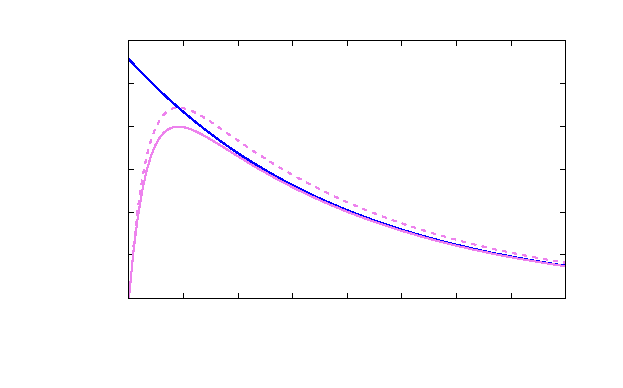
\includegraphics{transitori}}%
    \gplfronttext
  \end{picture}%
\endgroup

	\caption{Activitat del \( \mathsf{{}^{99}\text{Mo}} \) i del \( \mathsf{{}^{99}\text{Tc}} \) en funció del temps.}
	\label{fig:equilibri transitori}
\end{figure}
Considerem el cas d'equilibri secular, és a dir quan \( \lambda_X \ll \lambda_Y \). Aleshores tenim 
\begin{equation*}
	\frac{\lambda_X \lambda_Y}{\lambda_Y - \lambda_X} \approx \lambda_X.
\end{equation*}
Per tant, substituint a (\ref{eq:activitats}) tenim que 
\begin{equation*}
	A_Y(t) \approx \lambda_X N \left(e^{-\lambda_X t} - e^{-\lambda_Y t}\right) = \lambda_X N e^{-\lambda_X t} \left(1 - e^{(\lambda_X -\lambda_Y) t}\right) \approx \lambda_X N e^{-\lambda_X t}.
\end{equation*}
Per a l'última aproximació, observem que \( \lambda_X - \lambda_Y \approx -\lambda_Y \) en el règim en el que estem, i per tant el terme \( e^{(\lambda_X - \lambda_Y) t} \) decaurà ràpidament. Per tant, en l'equilibri tindrem que \( A_X = A_Y \). I a més, si el temps de mitja vida de \( X \) és molt gran comparat amb l'escala de temps que considerem, les dues activitats seran bàsicament constants un cop s'assoleixi l'equilibri.

Finalment, si \( \lambda_X > \lambda_Y \) aleshores l'activitat de \( X \) decaurà molt més depressa que la de \( Y \). Ja hem observat que en aquest cas \( A_Y/A_X \) no té límit finit, sino que tendeix a \( -\infty \), per tant no s'assolirà cap equilibri. 

\begin{figure}[htb]
	\center
	% GNUPLOT: LaTeX picture with Postscript
\begingroup
\sffamily \footnotesize
  \makeatletter
  \providecommand\color[2][]{%
    \GenericError{(gnuplot) \space\space\space\@spaces}{%
      Package color not loaded in conjunction with
      terminal option `colourtext'%
    }{See the gnuplot documentation for explanation.%
    }{Either use 'blacktext' in gnuplot or load the package
      color.sty in LaTeX.}%
    \renewcommand\color[2][]{}%
  }%
  \providecommand\includegraphics[2][]{%
    \GenericError{(gnuplot) \space\space\space\@spaces}{%
      Package graphicx or graphics not loaded%
    }{See the gnuplot documentation for explanation.%
    }{The gnuplot epslatex terminal needs graphicx.sty or graphics.sty.}%
    \renewcommand\includegraphics[2][]{}%
  }%
  \providecommand\rotatebox[2]{#2}%
  \@ifundefined{ifGPcolor}{%
    \newif\ifGPcolor
    \GPcolortrue
  }{}%
  \@ifundefined{ifGPblacktext}{%
    \newif\ifGPblacktext
    \GPblacktextfalse
  }{}%
  % define a \g@addto@macro without @ in the name:
  \let\gplgaddtomacro\g@addto@macro
  % define empty templates for all commands taking text:
  \gdef\gplbacktext{}%
  \gdef\gplfronttext{}%
  \makeatother
  \ifGPblacktext
    % no textcolor at all
    \def\colorrgb#1{}%
    \def\colorgray#1{}%
  \else
    % gray or color?
    \ifGPcolor
      \def\colorrgb#1{\color[rgb]{#1}}%
      \def\colorgray#1{\color[gray]{#1}}%
      \expandafter\def\csname LTw\endcsname{\color{white}}%
      \expandafter\def\csname LTb\endcsname{\color{black}}%
      \expandafter\def\csname LTa\endcsname{\color{black}}%
      \expandafter\def\csname LT0\endcsname{\color[rgb]{1,0,0}}%
      \expandafter\def\csname LT1\endcsname{\color[rgb]{0,1,0}}%
      \expandafter\def\csname LT2\endcsname{\color[rgb]{0,0,1}}%
      \expandafter\def\csname LT3\endcsname{\color[rgb]{1,0,1}}%
      \expandafter\def\csname LT4\endcsname{\color[rgb]{0,1,1}}%
      \expandafter\def\csname LT5\endcsname{\color[rgb]{1,1,0}}%
      \expandafter\def\csname LT6\endcsname{\color[rgb]{0,0,0}}%
      \expandafter\def\csname LT7\endcsname{\color[rgb]{1,0.3,0}}%
      \expandafter\def\csname LT8\endcsname{\color[rgb]{0.5,0.5,0.5}}%
    \else
      % gray
      \def\colorrgb#1{\color{black}}%
      \def\colorgray#1{\color[gray]{#1}}%
      \expandafter\def\csname LTw\endcsname{\color{white}}%
      \expandafter\def\csname LTb\endcsname{\color{black}}%
      \expandafter\def\csname LTa\endcsname{\color{black}}%
      \expandafter\def\csname LT0\endcsname{\color{black}}%
      \expandafter\def\csname LT1\endcsname{\color{black}}%
      \expandafter\def\csname LT2\endcsname{\color{black}}%
      \expandafter\def\csname LT3\endcsname{\color{black}}%
      \expandafter\def\csname LT4\endcsname{\color{black}}%
      \expandafter\def\csname LT5\endcsname{\color{black}}%
      \expandafter\def\csname LT6\endcsname{\color{black}}%
      \expandafter\def\csname LT7\endcsname{\color{black}}%
      \expandafter\def\csname LT8\endcsname{\color{black}}%
    \fi
  \fi
    \setlength{\unitlength}{0.0500bp}%
    \ifx\gptboxheight\undefined%
      \newlength{\gptboxheight}%
      \newlength{\gptboxwidth}%
      \newsavebox{\gptboxtext}%
    \fi%
    \setlength{\fboxrule}{0.5pt}%
    \setlength{\fboxsep}{1pt}%
\begin{picture}(5668.00,3400.00)%
    \gplgaddtomacro\gplbacktext{%
      \csname LTb\endcsname%%
      \put(1078,704){\makebox(0,0)[r]{\strut{}$\mathsf{0}$}}%
      \put(1078,1058){\makebox(0,0)[r]{\strut{}$\mathsf{0.01}$}}%
      \put(1078,1411){\makebox(0,0)[r]{\strut{}$\mathsf{0.02}$}}%
      \put(1078,1765){\makebox(0,0)[r]{\strut{}$\mathsf{0.03}$}}%
      \put(1078,2118){\makebox(0,0)[r]{\strut{}$\mathsf{0.04}$}}%
      \put(1078,2472){\makebox(0,0)[r]{\strut{}$\mathsf{0.05}$}}%
      \put(1078,2825){\makebox(0,0)[r]{\strut{}$\mathsf{0.06}$}}%
      \put(1078,3179){\makebox(0,0)[r]{\strut{}$\mathsf{0.07}$}}%
      \put(1210,484){\makebox(0,0){\strut{}$\mathsf{0}$}}%
      \put(1887,484){\makebox(0,0){\strut{}$\mathsf{5}$}}%
      \put(2564,484){\makebox(0,0){\strut{}$\mathsf{10}$}}%
      \put(3241,484){\makebox(0,0){\strut{}$\mathsf{15}$}}%
      \put(3917,484){\makebox(0,0){\strut{}$\mathsf{20}$}}%
      \put(4594,484){\makebox(0,0){\strut{}$\mathsf{25}$}}%
      \put(5271,484){\makebox(0,0){\strut{}$\mathsf{30}$}}%
      \put(1345,2825){\makebox(0,0)[l]{\strut{}$\mathsf{ {}^{113}\text{Sn}}$}}%
      \put(1887,2472){\makebox(0,0)[l]{\strut{}$\mathsf{ {}^{113}\text{In}^{\ast}}$}}%
    }%
    \gplgaddtomacro\gplfronttext{%
      \csname LTb\endcsname%%
      \put(198,1941){\rotatebox{-270}{\makebox(0,0){\strut{}Activitat per nucli (\si{\micro Bq})}}}%
      \put(3240,154){\makebox(0,0){\strut{}Temps (h)}}%
    }%
    \gplbacktext
    \put(0,0){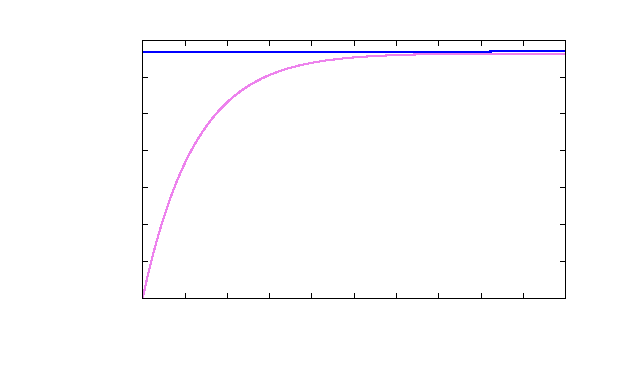
\includegraphics{secular}}%
    \gplfronttext
  \end{picture}%
\endgroup

	\caption{Activitat del \( \mathsf{{}^{113}\text{Sn}} \) i del \( \mathsf{{}^{113}\text{In}} \) en funció del temps.}
	\label{fig:equilibri secular}
\end{figure}
Com a exemple d'equilibri transitori podem considerar la següent cadena de desintegracions:
\begin{equation*}
	{}_{42}^{99} \mathrm{Mo} \xrightarrow{\beta^-} {}_{43}^{99} \mathrm{Tc}^{\ast} \xrightarrow{\gamma} {}_{43}^{99} \mathrm{Tc}.
\end{equation*}
La desintegració \( \beta^- \) del molibdè--99 en tecneci--99 excitat té un temps de mitja vida de \SI{67}{h}, per tant una constant de desintegració de \SI{0.01}{h^{-1}}. En canvi, l'estabilització del tecneci--99 a través d'una emissió \( \gamma \) té un temps de mitja vida de \SI{6}{h} i per tant una constant de desintegració de \SI{0.12}{h^{-1}}. A la figura \ref{fig:equilibri transitori} es mostra l'activitat de cada nucli en la cadena de desintegracions. Es pot veure que s'arriba a l'equilibri al voltant d'un dia, temps a partir del qual les dues activitats decauen al mateix ritme. Cal mencionar que un \num{10}\% de les desintegracions \( \beta^- \) del \( {}^{99}\text{Mo} \) tenen com a producte \( {}^{99}\text{Tc} \) i no \( {}^{99}\text{Tc}^{\ast} \) de manera que la contribució del \(  {}^{99}\text{Mo} \) al \( {}^{99}\text{Tc} \) es veu reduïda en aquest percentatge. La línia intermitent mostra l'activitat del tecneci sense la correcció, i la línia sòlida amb la correcció.


\begin{figure}[htb]
	\center
	% GNUPLOT: LaTeX picture with Postscript
\begingroup
\sffamily \footnotesize
  \makeatletter
  \providecommand\color[2][]{%
    \GenericError{(gnuplot) \space\space\space\@spaces}{%
      Package color not loaded in conjunction with
      terminal option `colourtext'%
    }{See the gnuplot documentation for explanation.%
    }{Either use 'blacktext' in gnuplot or load the package
      color.sty in LaTeX.}%
    \renewcommand\color[2][]{}%
  }%
  \providecommand\includegraphics[2][]{%
    \GenericError{(gnuplot) \space\space\space\@spaces}{%
      Package graphicx or graphics not loaded%
    }{See the gnuplot documentation for explanation.%
    }{The gnuplot epslatex terminal needs graphicx.sty or graphics.sty.}%
    \renewcommand\includegraphics[2][]{}%
  }%
  \providecommand\rotatebox[2]{#2}%
  \@ifundefined{ifGPcolor}{%
    \newif\ifGPcolor
    \GPcolortrue
  }{}%
  \@ifundefined{ifGPblacktext}{%
    \newif\ifGPblacktext
    \GPblacktextfalse
  }{}%
  % define a \g@addto@macro without @ in the name:
  \let\gplgaddtomacro\g@addto@macro
  % define empty templates for all commands taking text:
  \gdef\gplbacktext{}%
  \gdef\gplfronttext{}%
  \makeatother
  \ifGPblacktext
    % no textcolor at all
    \def\colorrgb#1{}%
    \def\colorgray#1{}%
  \else
    % gray or color?
    \ifGPcolor
      \def\colorrgb#1{\color[rgb]{#1}}%
      \def\colorgray#1{\color[gray]{#1}}%
      \expandafter\def\csname LTw\endcsname{\color{white}}%
      \expandafter\def\csname LTb\endcsname{\color{black}}%
      \expandafter\def\csname LTa\endcsname{\color{black}}%
      \expandafter\def\csname LT0\endcsname{\color[rgb]{1,0,0}}%
      \expandafter\def\csname LT1\endcsname{\color[rgb]{0,1,0}}%
      \expandafter\def\csname LT2\endcsname{\color[rgb]{0,0,1}}%
      \expandafter\def\csname LT3\endcsname{\color[rgb]{1,0,1}}%
      \expandafter\def\csname LT4\endcsname{\color[rgb]{0,1,1}}%
      \expandafter\def\csname LT5\endcsname{\color[rgb]{1,1,0}}%
      \expandafter\def\csname LT6\endcsname{\color[rgb]{0,0,0}}%
      \expandafter\def\csname LT7\endcsname{\color[rgb]{1,0.3,0}}%
      \expandafter\def\csname LT8\endcsname{\color[rgb]{0.5,0.5,0.5}}%
    \else
      % gray
      \def\colorrgb#1{\color{black}}%
      \def\colorgray#1{\color[gray]{#1}}%
      \expandafter\def\csname LTw\endcsname{\color{white}}%
      \expandafter\def\csname LTb\endcsname{\color{black}}%
      \expandafter\def\csname LTa\endcsname{\color{black}}%
      \expandafter\def\csname LT0\endcsname{\color{black}}%
      \expandafter\def\csname LT1\endcsname{\color{black}}%
      \expandafter\def\csname LT2\endcsname{\color{black}}%
      \expandafter\def\csname LT3\endcsname{\color{black}}%
      \expandafter\def\csname LT4\endcsname{\color{black}}%
      \expandafter\def\csname LT5\endcsname{\color{black}}%
      \expandafter\def\csname LT6\endcsname{\color{black}}%
      \expandafter\def\csname LT7\endcsname{\color{black}}%
      \expandafter\def\csname LT8\endcsname{\color{black}}%
    \fi
  \fi
    \setlength{\unitlength}{0.0500bp}%
    \ifx\gptboxheight\undefined%
      \newlength{\gptboxheight}%
      \newlength{\gptboxwidth}%
      \newsavebox{\gptboxtext}%
    \fi%
    \setlength{\fboxrule}{0.5pt}%
    \setlength{\fboxsep}{1pt}%
\begin{picture}(5668.00,3400.00)%
    \gplgaddtomacro\gplbacktext{%
      \csname LTb\endcsname%%
      \put(814,704){\makebox(0,0)[r]{\strut{}$\mathsf{0}$}}%
      \put(814,1013){\makebox(0,0)[r]{\strut{}$\mathsf{5}$}}%
      \put(814,1323){\makebox(0,0)[r]{\strut{}$\mathsf{10}$}}%
      \put(814,1632){\makebox(0,0)[r]{\strut{}$\mathsf{15}$}}%
      \put(814,1942){\makebox(0,0)[r]{\strut{}$\mathsf{20}$}}%
      \put(814,2251){\makebox(0,0)[r]{\strut{}$\mathsf{25}$}}%
      \put(814,2560){\makebox(0,0)[r]{\strut{}$\mathsf{30}$}}%
      \put(814,2870){\makebox(0,0)[r]{\strut{}$\mathsf{35}$}}%
      \put(814,3179){\makebox(0,0)[r]{\strut{}$\mathsf{40}$}}%
      \put(946,484){\makebox(0,0){\strut{}$\mathsf{0}$}}%
      \put(1487,484){\makebox(0,0){\strut{}$\mathsf{5}$}}%
      \put(2027,484){\makebox(0,0){\strut{}$\mathsf{10}$}}%
      \put(2568,484){\makebox(0,0){\strut{}$\mathsf{15}$}}%
      \put(3109,484){\makebox(0,0){\strut{}$\mathsf{20}$}}%
      \put(3649,484){\makebox(0,0){\strut{}$\mathsf{25}$}}%
      \put(4190,484){\makebox(0,0){\strut{}$\mathsf{30}$}}%
      \put(4730,484){\makebox(0,0){\strut{}$\mathsf{35}$}}%
      \put(5271,484){\makebox(0,0){\strut{}$\mathsf{40}$}}%
      \put(1162,2684){\makebox(0,0)[l]{\strut{}$\mathsf{ {}^{210}\text{Bi}}$}}%
      \put(1162,890){\makebox(0,0)[l]{\strut{}$\mathsf{ {}^{210}\text{Po}}$}}%
    }%
    \gplgaddtomacro\gplfronttext{%
      \csname LTb\endcsname%%
      \put(198,1941){\rotatebox{-270}{\makebox(0,0){\strut{}Activitat per nucli (\si{\micro Bq})}}}%
      \put(3108,154){\makebox(0,0){\strut{}Temps (d)}}%
    }%
    \gplbacktext
    \put(0,0){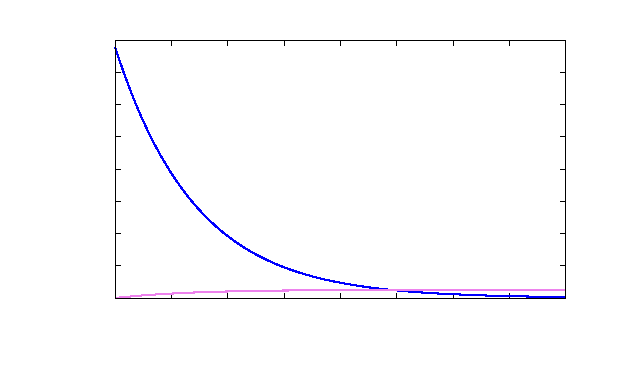
\includegraphics{no-equilibri}}%
    \gplfronttext
  \end{picture}%
\endgroup

	\caption{Activitat del \( \mathsf{{}^{210}\text{Bi}} \) i del \( \mathsf{{}^{210}\text{Po}} \) en funció del temps.}
	\label{fig:no equilibri}
\end{figure}
Un exemple d'equilibri transitori és la cadena següent:
\begin{equation*}
	{}^{113}_{50}\text{Sn} \xrightarrow{e^-} {}^{113}_{49}\text{In}^{\ast} \xrightarrow{\gamma} {}^{113}_{49}\text{In}
\end{equation*}
L'estany--113 es transforma en indi--113 excitat mitjançant una captura electrònica, i després s'estabilitza a través d'una emissió \( \gamma \). El primer procés té un temps de mitja vida de \SI{118}{d}, i el segon de \SI{1.7}{h}. Per tant tenen constants de desintegració \( \SI{5.9e-3}{d^{-1}} = \SI{2.4e-4}{h^{-1}} \) i \SI{0.41}{h^{-1}} respectivament. Tal i com es pot apreciar a la figura \ref{fig:equilibri secular}, l'activitat de l'indi és bàsicament idèntica a la de l'estany passades unes \SI{15}{h}, i la de l'estany es manté bàsicament constant en tot aquest temps. 

Finalment, considerem la següent cadena de desintegracions:
\begin{equation*}
	{}^{210}_{83}\text{Bi} \xrightarrow{\beta^-} {}^{210}_{84}\text{Po} \xrightarrow{\alpha} {}^{206}_{82}\text{Pb}
\end{equation*}
El bismut--210 decau amb un temps de mitja vida de \SI{5.01}{d}, i el poloni--210 decau amb un temps de mitja vida de \SI{138}{d}. El producte final, el plom--82 és estable. Les constants de desintegració, doncs, són \SI{0,14}{d^{-1}} i \SI{5e-3}{d^{-1}}. Per tant estem en la situació en la que no s'assoleix un equilibri. Això es pot apreciar a la figura \ref{fig:no equilibri}.

\end{document}
